\part{Technical assessment of water hammer for expansion loops}
\section{Frequency of the water hammer pressure fluctuation in a pipe}
\subsection{MATLAB script}
\subsubsection{Pressure fluctuation and Joukowski prediction}
The calculation for maximum magnitude of the water hammer pulse is \eqref{jk1}. This is also known as the Joukowski equation.
\begin{gather}\label{jk1}
    \Delta p = \rho a_0 \Delta v\, (\si{\pascal})
\end{gather}
where $\Delta p$ is the change in pressure, $\rho$ is the fluid density, $a_0$ is the sonic velocity in the pipe and $\Delta v$ is the change in fluid velocity. The sonic velocity $a$ can be determined through \eqref{sonic1}, which is a modified version of Hooke's law. This allows to take into account the stiffness of the fluid and pipe wall. This assumes that our flow is free of of bubbles and is uniformly LNG and the pipe is sufficiently thin ($D/\tau > 40$) \cite{Watters1984AnalysisAC}.
\begin{gather}\label{sonic1}
    \frac{1}{a^2} = \frac{1}{c^2} + \frac{\rho D }{\tau E}
\end{gather}
where $c$ is the speed of sound in the fluid, $\rho$ is fluid density, $D$ is pipe internal diameter, $\tau$ is wall thickness of pipe and $E$ is Young's Modulus of pipe. Running the MATLAB script with the values shown in Table \ref{matlabScriptVals}, Figure \ref{pressure1} was generated.

The pressure values at the first peak of the rise were chosen to find the maximum pressure differential. A settled pressure differential value was also found (shown in Figure \ref{pressure2}). Table \ref{matlabResults} shows the maximum pressure differentials for each index point ($s$- value: point along length of pipe from valve) and the pressure differential of the settled value.

The Joukowski prediction makes assumptions in order to calculate a value for our pressure differential. This may explain the discrepancy we see for our differential values. For example, the Joukowski prediction does not account for frictional losses within the system. We also assume there is no column separation, cavitation or any other fluid effects.

\begin{table}[H]
    \centering
    \begin{tabular}{@{}rr@{}}
        \toprule
        \textbf{Parameter}     & \textbf{Value}                       \\
        \midrule
        $c$                    & \SI{1100}{\meter\per\second}         \\
        $\rho$                 & \SI{455}{\kilo\gram\per\meter\cubed} \\
        $D$                    & \SI{793.94}{\milli\meter}            \\
        $\tau$                 & \SI{19.06}{\milli\meter}             \\
        $E$                    & \SI{200}{\giga\pascal}               \\
        $\Delta v$             & \SI{1.5}{\meter\per\second}          \\
        $a_0$                  & \SI{1041.89}{\meter\per\second}      \\
        $\Delta p_{joukowski}$ & \SI{711087}{\pascal}                 \\
        \bottomrule
    \end{tabular}
    \caption{Values for Joukowski Prediction and calculated pressure differential.}
    \label{matlabScriptVals}
\end{table}

\begin{figure}[H]
    \centering
    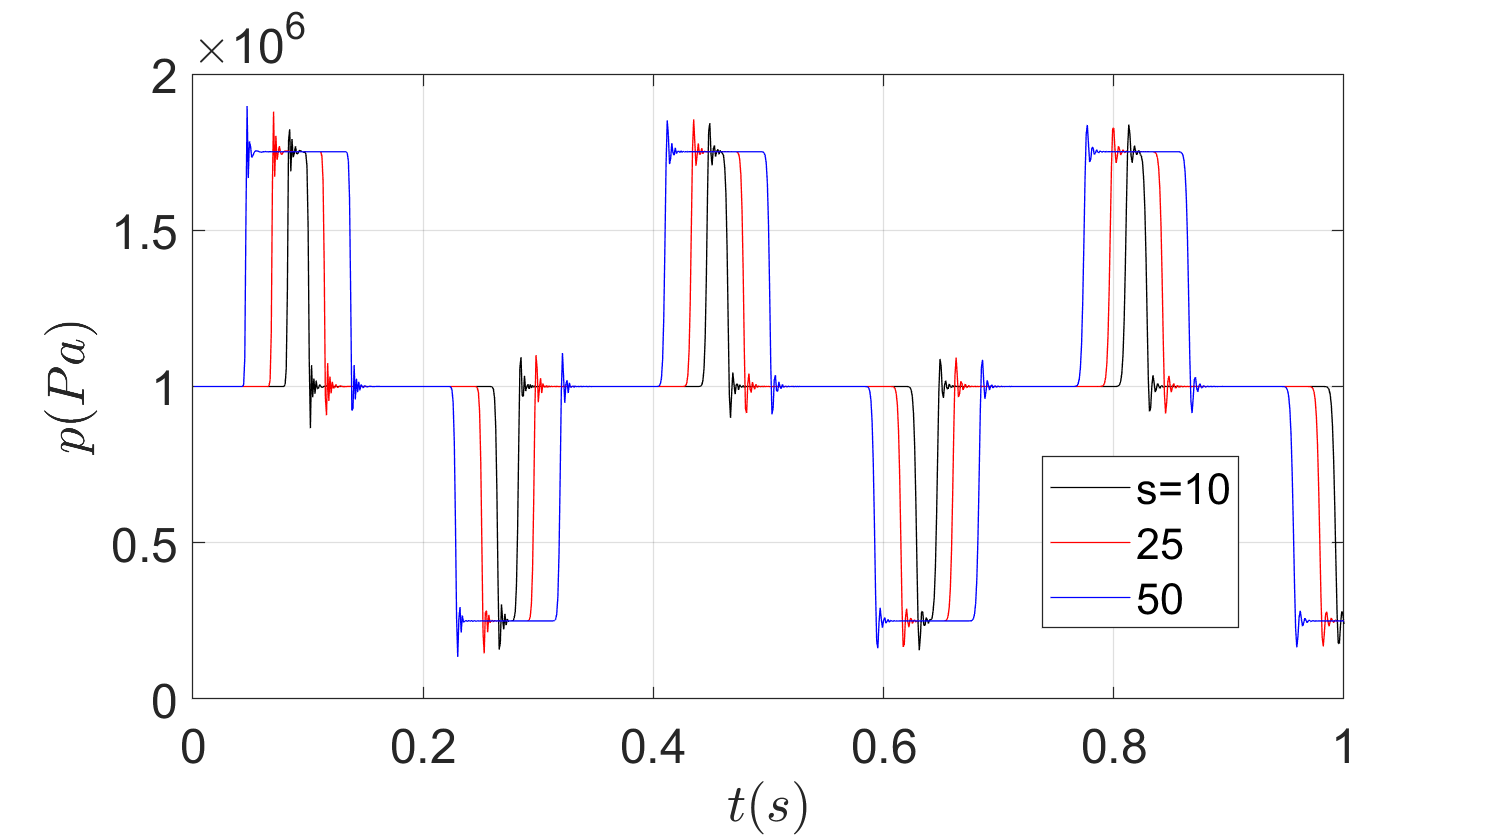
\includegraphics[width = 0.9 \textwidth]{img/fig1.png}
    \caption{MATLAB script results showing pressure against time for $s=10,\,25,\,\SI{50}{\meter}$.}
    \label{pressure1}
\end{figure}

\begin{figure}[H]
    \centering
    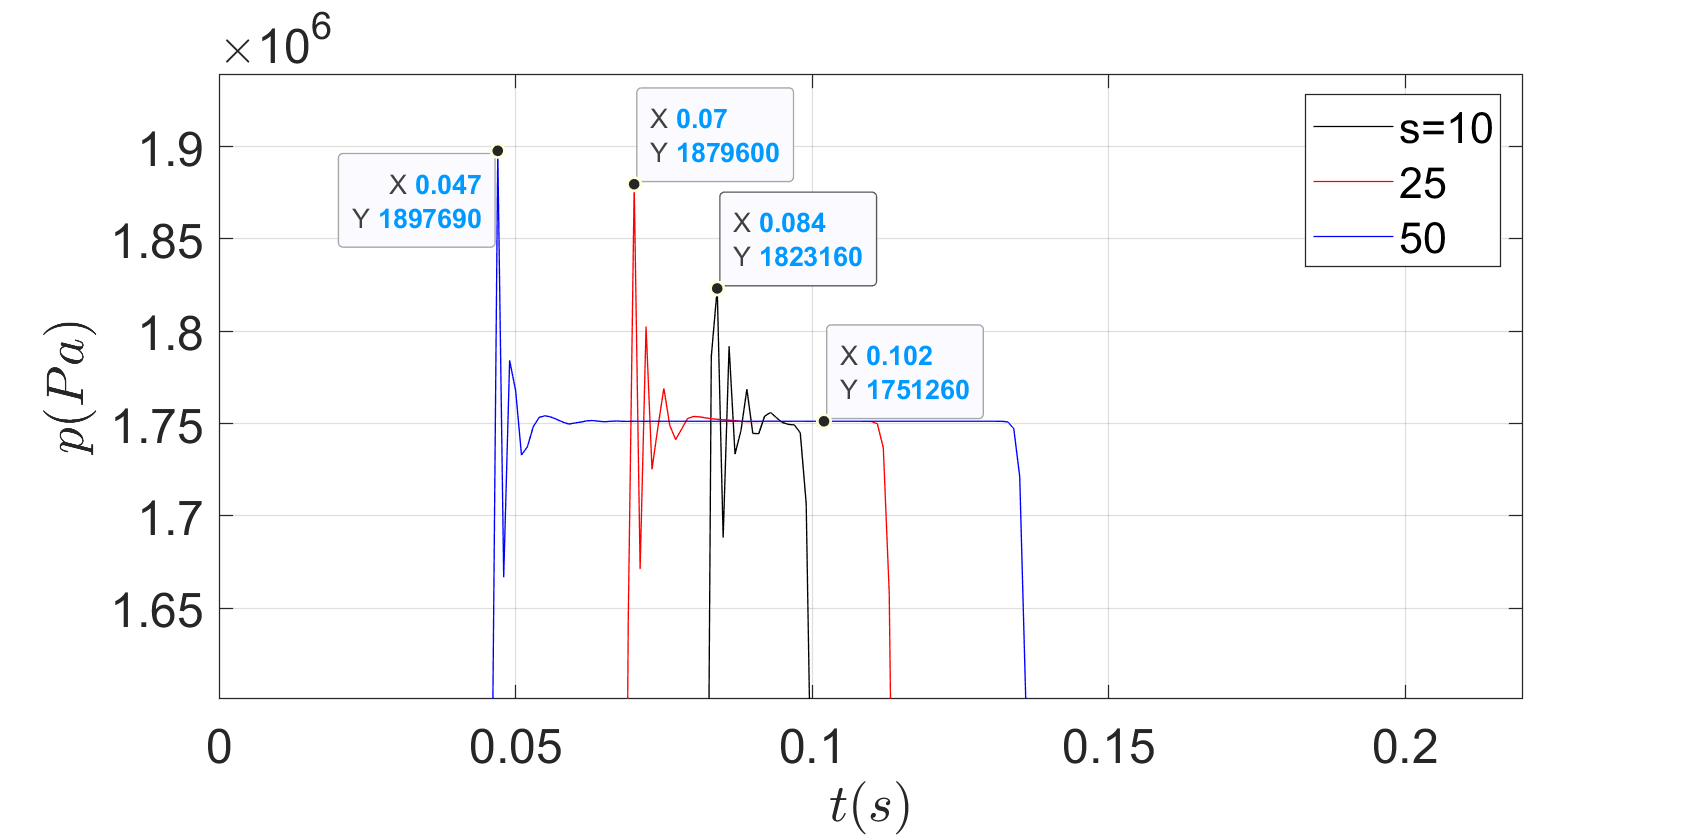
\includegraphics[width = 0.9 \textwidth]{img/fig3.png}
    \caption{Index points for finding maximum pressure differential and settled pressure differential.}
    \label{pressure2}
\end{figure}

\begin{table}[H]
    \centering
    \begin{tabular}{@{}rrr@{}}
        \toprule
        \textbf{$s$- value} & \textbf{Maximum pressure }         & \textbf{Percentage difference}  \\
                            & \textbf{differential}/\si{\pascal} & \textbf{compared to analytical} \\
        \midrule
        10                  & 823160                             & 15.76\%                         \\
        25                  & 879600                             & 23.70\%                         \\
        50                  & 897690                             & 26.24\%                         \\
        Settled value       & 751260                             & 5.64\%                          \\
        \bottomrule
    \end{tabular}
    \caption{Pressure differentials for indexed $s$- values and settled values.}
    \label{matlabResults}
\end{table}
\subsubsection{Frequencies associated with pressure fluctiation and analytical prediction}
An analytical result for the frequencies of the pressure fluctuation can be found using \eqref{freq1} \cite{piping}.
\begin{gather}\label{freq1}
    T = \frac{1}{f} = \frac{2L}{c} = \frac{2\cdot s}{1100}
\end{gather}
Indexing the values found in our MATLAB result, we can find the frequencies of the pressure fluctuation in Table \ref{freq2}. The index points were selected as the first peak of the rise and the first peak of the return to \SI{1}{\mega\pascal}. The time between these points represents the duration of the pressure rise from the wave propagating past a particular point in the pipe. The results show a relatively low percentage error. Our discrepancy may stem from a lack of temporal resolution, as we are only using a time step of \SI{1e-3}{\second}. A higher time-step may allow us to accurately find the value of the first peaks.
\begin{table}[H]
    \centering
    \begin{tabular}{@{}rrrr@{}}
        \toprule
        \textbf{$s$- value} & \multicolumn{2}{c}{\textbf{Frequency}/\si{\hertz}} & \textbf{Percentage}                       \\
                            & \textbf{MATLAB}                                    & \textbf{Analytical} & \textbf{difference} \\
        \midrule
        10                  & 10.99                                              & 11                  & 0.09\%              \\
        25                  & 21.74                                              & 22                  & 1.18\%              \\
        50                  & 55.56                                              & 55                  & 1.02\%              \\
        \bottomrule
    \end{tabular}
    \caption{Frequency of pressure fluctuation.}
    \label{freq2}
\end{table}
\subsection{Force analysis}
\subsubsection{Force acting on bend due to reflection of pressure wave}
Using MATLAB, the forces acting on each bend of the loop were calculated. Figure \ref{force1} shows a plot of the forces from the first reflection of the pressure wave. Figure \ref{force2} shows the forces on each bend for the given time period from each reflection of the pressure wave.

\begin{figure}[H]
    \centering
    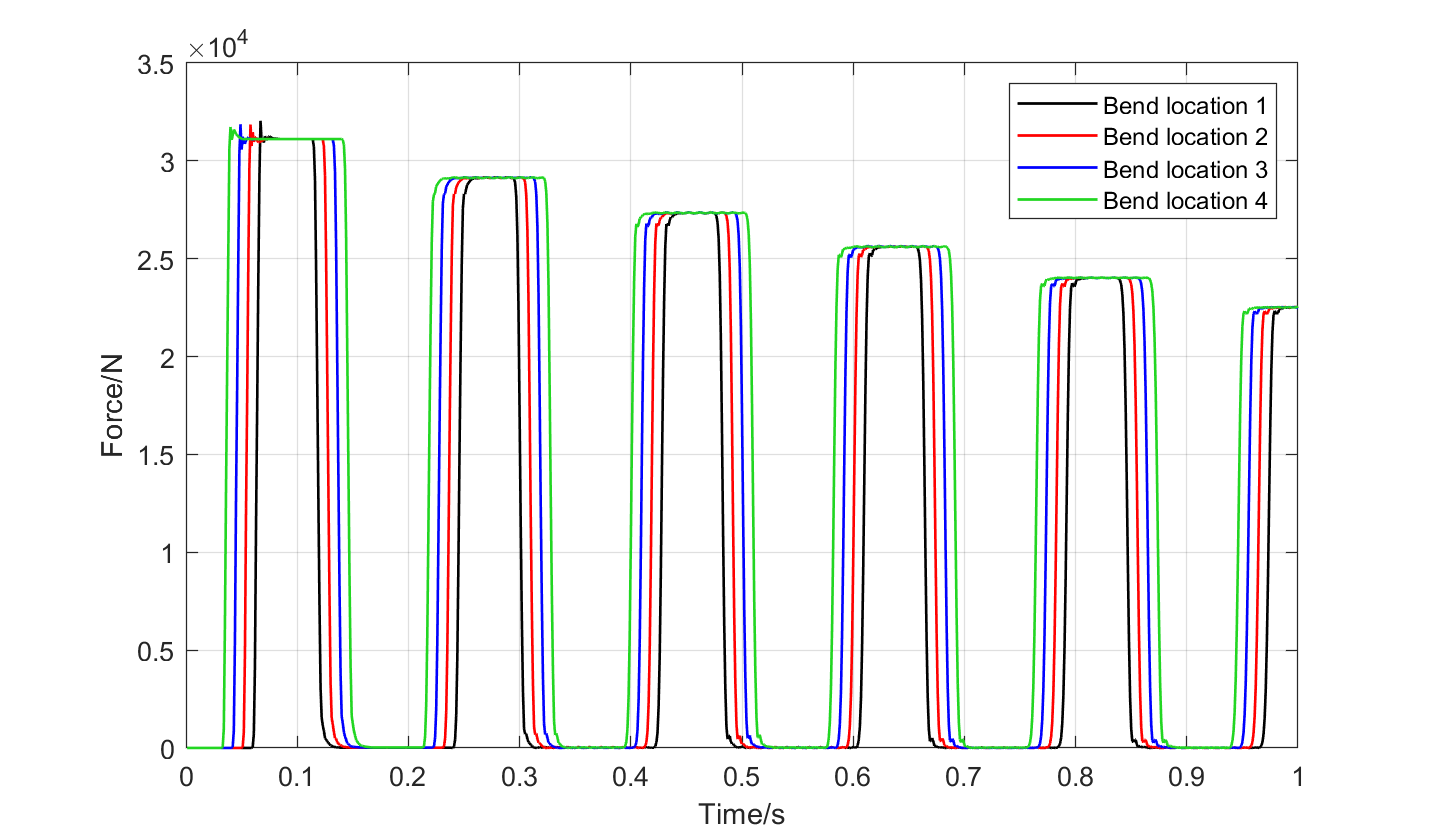
\includegraphics[width = 0.9 \textwidth]{img/fig6.png}
    \caption{Forces on each bend from reflections of pressure wave over the time period.}
    \label{force2}
\end{figure}

\begin{figure}[H]
    \centering
    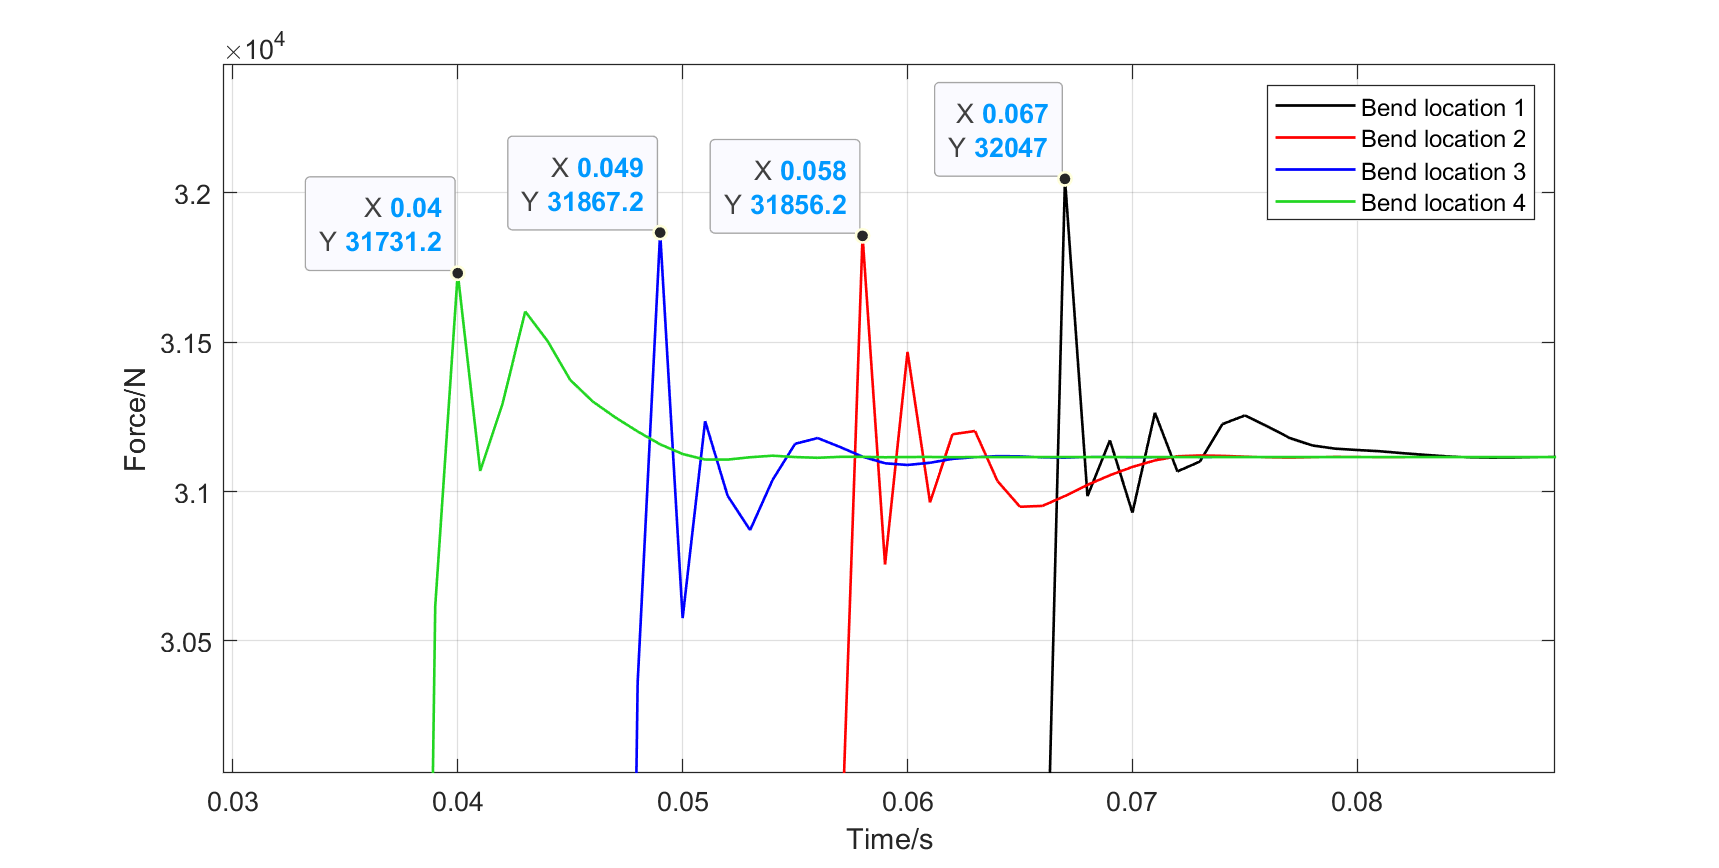
\includegraphics[width = 0.9 \textwidth]{img/fig5.png}
    \caption{Forces on each bend from first reflection of pressure wave.}
    \label{force1}
\end{figure}

\subsubsection{Direction of total force on expansion loop}
\section{Modal analysis of expansion loop}
\subsection{Modal analysis of a cantilevered pipe}
In order to conduct our ANSYS analysis, we need to find the effective pipe density, we can use \eqref{rhoEff}.
\begin{gather}\label{rhoEff}
    \rho_{eff} = \rho_s + \rho_{LNG}\left(\frac{d_i^2}{d_e^2 - d_i^2}\right)
\end{gather}
Table \ref{modalParams} shows the values used in the ANSYS simulations.
\begin{table}[H]
    \centering
    \begin{tabular}{@{}rr@{}}
        \toprule
        \textbf{Parameter} & \textbf{Value}                            \\
        \midrule
        $d_i$              & \SI{793.94}{\milli\meter}                 \\
        $d_e$              & \SI{813}{\milli\meter}                    \\
        $\rho_s$           & \SI{7850}{\kilo\gram\per\meter\cubed}     \\
        $\rho_{LNG}$       & \SI{455}{\kilo\gram\per\meter\cubed}      \\
        $\rho_{eff}$       & \SI{17214.06}{\kilo\gram\per\meter\cubed} \\
        \bottomrule
    \end{tabular}
    \caption{Values for cantilevered beam analysis in ANSYS.}
    \label{modalParams}
\end{table}
\subsubsection{List of unique frequencies \& mesh sensitivity test}
Table \ref{modal1} shows values of the modal frequencies for a cantilevered pipe with lengths $L = 10,\,20,\,\SI{30}{\meter}$. For the theoretical values, we can calculate the bending moment of a cantilevered beam using \eqref{fn1}.
\begin{gather}
    f_n = \frac{\alpha_n^2}{2\pi}\left(\frac{EI}{AL^4}\right)^{\frac{1}{2}}\label{fn1}\\
    I = \frac{A}{16}\left(d^2_e + d^2_i\right)
\end{gather}
where coefficient $\alpha_n$ values were found in literature. The theoretical values were calculated using MATLAB (Appendix \ref{app:modalFreq1})
\begin{table}[H]
    \centering
    \begin{tabular}{@{}rrrrrrr@{}}
        \toprule
        \textbf{Mode} & \multicolumn{6}{c}{\textbf{Frequency/Hz}}                                                                                                                                              \\
                      & \textbf{ANSYS}                            & \textbf{Theory}                           & \textbf{ANSYS}                            & \textbf{Theory} & \textbf{ANSYS} & \textbf{Theory} \\
                      & \multicolumn{2}{c}{$L = \SI{4}{\meter}$}  & \multicolumn{2}{c}{$L = \SI{10}{\meter}$} & \multicolumn{2}{c}{$L = \SI{20}{\meter}$}                                                      \\
        \midrule
        1             & 31.65                                     & 33.86                                     & 5.35                                      & 5.42            & 1.35           & 1.35            \\
        2             & 149.93                                    & 212.23                                    & 31.49                                     & 33.96           & 8.37           & 8.49            \\
        3             & 332.21                                    & 594.32                                    & 80.99                                     & 95.09           & 22.69          & 23.77           \\
        4             & 521.06                                    & 1164.66                                   & 143.54                                    & 186.35          & 42.93          & 46.59           \\
        5             & 712.09                                    & 1925.06                                   & 214.08                                    & 308.01          & 68.06          & 77.00           \\
        6             & 857.22                                    & 2875.85                                   & 289.12                                    & 460.14          & 97.07          & 115.03          \\
        \bottomrule
    \end{tabular}
    \caption{Table to show values of modal frequencies for a cantilever beam of length $L = 10,\,20,\,\SI{30}{\meter}$, compared to theoretical values.}
    \label{modal1}
\end{table}
A mesh sensitivity test was conducted using the $L=\SI{4}{\meter}$ case. The element size was varied from \SI{0.5}{\meter} to \SI{0.01}{\meter} and the modal frequencies were found. By taking the frequency of a particular mode and element size and comparing it to the frequency found in the simulation with element size \SI{0.01}{\meter} (for the same mode), a percentage difference was calculated. Figure \ref{mesh1} shows how frequency values converge. We see that the percentage difference in frequency for element size \SI{0.125}{\meter} and smaller is negligible. Hence, for the simulations conducted, a mesh size of \SI{0.125}{\meter} was used.
\begin{figure}[H]
    \centering
    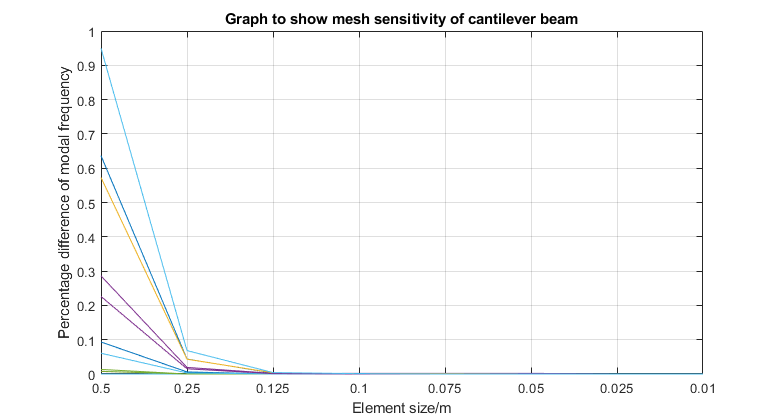
\includegraphics[width = 0.9\textwidth]{img/fig4.png}
    \caption{Mesh sensitivity test results. Conducted on a beam with length $L=\SI{4}{\meter}$.}
    \label{mesh1}
\end{figure}
\subsubsection{Differences and similarities between theoretical and calculated modes}
Using MATLAB, the percentage difference between the ANSYS values and the theoeretical values was found. This is shown in Table \ref{percDiffs}.
\begin{table}[H]
    \centering
    \begin{tabular}{@{}rrrr@{}}
        \toprule
        \textbf{Mode} & \multicolumn{3}{c}{\textbf{Percentage difference (\%)}}                                                 \\
                      & $L = \SI{4}{\meter}$                                    & $L = \SI{10}{\meter}$ & $L = \SI{20}{\meter}$ \\
        \midrule
        1             & 7.00                                                    & 1.27                  & 0.34                  \\
        2             & 41.56                                                   & 7.84                  & 1.43                  \\
        3             & 78.90                                                   & 17.41                 & 4.77                  \\
        4             & 123.52                                                  & 29.82                 & 8.52                  \\
        5             & 170.33                                                  & 43.88                 & 13.14                 \\
        6             & 235.49                                                  & 59.15                 & 18.51                 \\ \bottomrule
    \end{tabular}
    \caption{Table to show percentage difference between ANSYS modal frequencies and theoretical values.}
    \label{percDiffs}
\end{table}
We find that for lower $L$- values the modal frequencies are higher in our ANSYS simulation. This trend matches with the theoretical values, where modal frequency decreases as a function of $L$. For the first mode, we find that ANSYS and theory values are closely matched with single digit or decimal percentage difference. For higher modes, the percentage difference increases substantially. As $L$ increases, our percentage difference between ANSYS and theoretical values decreases. As the mode number increases, the percentage difference increases.

As we are using the Euler-Bernoulli theorem to calculate our theory values, the assumptions made can potentially explain the discrepancy between our modal frequency values. One such assumption is that plane sections remain plane. We know that for higher modes, the beam undergoes a larger displacement, as more sections of the beam are displaced from the normal axis. This large displacement results in plane sections no longer remaining plane, making our assumption invalid for higher modes.
\subsection{Modal analysis of an expansion loop}
\section{Discussion and context}
\bibliographystyle{unsrtnat}
\bibliography{RefsB.bib}